% Options for packages loaded elsewhere
\PassOptionsToPackage{unicode}{hyperref}
\PassOptionsToPackage{hyphens}{url}
\PassOptionsToPackage{dvipsnames,svgnames,x11names}{xcolor}
%
\documentclass[
  letterpaper,
  DIV=11,
  numbers=noendperiod]{scrartcl}

\usepackage{amsmath,amssymb}
\usepackage{iftex}
\ifPDFTeX
  \usepackage[T1]{fontenc}
  \usepackage[utf8]{inputenc}
  \usepackage{textcomp} % provide euro and other symbols
\else % if luatex or xetex
  \usepackage{unicode-math}
  \defaultfontfeatures{Scale=MatchLowercase}
  \defaultfontfeatures[\rmfamily]{Ligatures=TeX,Scale=1}
\fi
\usepackage{lmodern}
\ifPDFTeX\else  
    % xetex/luatex font selection
\fi
% Use upquote if available, for straight quotes in verbatim environments
\IfFileExists{upquote.sty}{\usepackage{upquote}}{}
\IfFileExists{microtype.sty}{% use microtype if available
  \usepackage[]{microtype}
  \UseMicrotypeSet[protrusion]{basicmath} % disable protrusion for tt fonts
}{}
\makeatletter
\@ifundefined{KOMAClassName}{% if non-KOMA class
  \IfFileExists{parskip.sty}{%
    \usepackage{parskip}
  }{% else
    \setlength{\parindent}{0pt}
    \setlength{\parskip}{6pt plus 2pt minus 1pt}}
}{% if KOMA class
  \KOMAoptions{parskip=half}}
\makeatother
\usepackage{xcolor}
\setlength{\emergencystretch}{3em} % prevent overfull lines
\setcounter{secnumdepth}{-\maxdimen} % remove section numbering
% Make \paragraph and \subparagraph free-standing
\ifx\paragraph\undefined\else
  \let\oldparagraph\paragraph
  \renewcommand{\paragraph}[1]{\oldparagraph{#1}\mbox{}}
\fi
\ifx\subparagraph\undefined\else
  \let\oldsubparagraph\subparagraph
  \renewcommand{\subparagraph}[1]{\oldsubparagraph{#1}\mbox{}}
\fi

\usepackage{color}
\usepackage{fancyvrb}
\newcommand{\VerbBar}{|}
\newcommand{\VERB}{\Verb[commandchars=\\\{\}]}
\DefineVerbatimEnvironment{Highlighting}{Verbatim}{commandchars=\\\{\}}
% Add ',fontsize=\small' for more characters per line
\usepackage{framed}
\definecolor{shadecolor}{RGB}{241,243,245}
\newenvironment{Shaded}{\begin{snugshade}}{\end{snugshade}}
\newcommand{\AlertTok}[1]{\textcolor[rgb]{0.68,0.00,0.00}{#1}}
\newcommand{\AnnotationTok}[1]{\textcolor[rgb]{0.37,0.37,0.37}{#1}}
\newcommand{\AttributeTok}[1]{\textcolor[rgb]{0.40,0.45,0.13}{#1}}
\newcommand{\BaseNTok}[1]{\textcolor[rgb]{0.68,0.00,0.00}{#1}}
\newcommand{\BuiltInTok}[1]{\textcolor[rgb]{0.00,0.23,0.31}{#1}}
\newcommand{\CharTok}[1]{\textcolor[rgb]{0.13,0.47,0.30}{#1}}
\newcommand{\CommentTok}[1]{\textcolor[rgb]{0.37,0.37,0.37}{#1}}
\newcommand{\CommentVarTok}[1]{\textcolor[rgb]{0.37,0.37,0.37}{\textit{#1}}}
\newcommand{\ConstantTok}[1]{\textcolor[rgb]{0.56,0.35,0.01}{#1}}
\newcommand{\ControlFlowTok}[1]{\textcolor[rgb]{0.00,0.23,0.31}{#1}}
\newcommand{\DataTypeTok}[1]{\textcolor[rgb]{0.68,0.00,0.00}{#1}}
\newcommand{\DecValTok}[1]{\textcolor[rgb]{0.68,0.00,0.00}{#1}}
\newcommand{\DocumentationTok}[1]{\textcolor[rgb]{0.37,0.37,0.37}{\textit{#1}}}
\newcommand{\ErrorTok}[1]{\textcolor[rgb]{0.68,0.00,0.00}{#1}}
\newcommand{\ExtensionTok}[1]{\textcolor[rgb]{0.00,0.23,0.31}{#1}}
\newcommand{\FloatTok}[1]{\textcolor[rgb]{0.68,0.00,0.00}{#1}}
\newcommand{\FunctionTok}[1]{\textcolor[rgb]{0.28,0.35,0.67}{#1}}
\newcommand{\ImportTok}[1]{\textcolor[rgb]{0.00,0.46,0.62}{#1}}
\newcommand{\InformationTok}[1]{\textcolor[rgb]{0.37,0.37,0.37}{#1}}
\newcommand{\KeywordTok}[1]{\textcolor[rgb]{0.00,0.23,0.31}{#1}}
\newcommand{\NormalTok}[1]{\textcolor[rgb]{0.00,0.23,0.31}{#1}}
\newcommand{\OperatorTok}[1]{\textcolor[rgb]{0.37,0.37,0.37}{#1}}
\newcommand{\OtherTok}[1]{\textcolor[rgb]{0.00,0.23,0.31}{#1}}
\newcommand{\PreprocessorTok}[1]{\textcolor[rgb]{0.68,0.00,0.00}{#1}}
\newcommand{\RegionMarkerTok}[1]{\textcolor[rgb]{0.00,0.23,0.31}{#1}}
\newcommand{\SpecialCharTok}[1]{\textcolor[rgb]{0.37,0.37,0.37}{#1}}
\newcommand{\SpecialStringTok}[1]{\textcolor[rgb]{0.13,0.47,0.30}{#1}}
\newcommand{\StringTok}[1]{\textcolor[rgb]{0.13,0.47,0.30}{#1}}
\newcommand{\VariableTok}[1]{\textcolor[rgb]{0.07,0.07,0.07}{#1}}
\newcommand{\VerbatimStringTok}[1]{\textcolor[rgb]{0.13,0.47,0.30}{#1}}
\newcommand{\WarningTok}[1]{\textcolor[rgb]{0.37,0.37,0.37}{\textit{#1}}}

\providecommand{\tightlist}{%
  \setlength{\itemsep}{0pt}\setlength{\parskip}{0pt}}\usepackage{longtable,booktabs,array}
\usepackage{calc} % for calculating minipage widths
% Correct order of tables after \paragraph or \subparagraph
\usepackage{etoolbox}
\makeatletter
\patchcmd\longtable{\par}{\if@noskipsec\mbox{}\fi\par}{}{}
\makeatother
% Allow footnotes in longtable head/foot
\IfFileExists{footnotehyper.sty}{\usepackage{footnotehyper}}{\usepackage{footnote}}
\makesavenoteenv{longtable}
\usepackage{graphicx}
\makeatletter
\def\maxwidth{\ifdim\Gin@nat@width>\linewidth\linewidth\else\Gin@nat@width\fi}
\def\maxheight{\ifdim\Gin@nat@height>\textheight\textheight\else\Gin@nat@height\fi}
\makeatother
% Scale images if necessary, so that they will not overflow the page
% margins by default, and it is still possible to overwrite the defaults
% using explicit options in \includegraphics[width, height, ...]{}
\setkeys{Gin}{width=\maxwidth,height=\maxheight,keepaspectratio}
% Set default figure placement to htbp
\makeatletter
\def\fps@figure{htbp}
\makeatother

\KOMAoption{captions}{tableheading}
\makeatletter
\makeatother
\makeatletter
\makeatother
\makeatletter
\@ifpackageloaded{caption}{}{\usepackage{caption}}
\AtBeginDocument{%
\ifdefined\contentsname
  \renewcommand*\contentsname{Table of contents}
\else
  \newcommand\contentsname{Table of contents}
\fi
\ifdefined\listfigurename
  \renewcommand*\listfigurename{List of Figures}
\else
  \newcommand\listfigurename{List of Figures}
\fi
\ifdefined\listtablename
  \renewcommand*\listtablename{List of Tables}
\else
  \newcommand\listtablename{List of Tables}
\fi
\ifdefined\figurename
  \renewcommand*\figurename{Figure}
\else
  \newcommand\figurename{Figure}
\fi
\ifdefined\tablename
  \renewcommand*\tablename{Table}
\else
  \newcommand\tablename{Table}
\fi
}
\@ifpackageloaded{float}{}{\usepackage{float}}
\floatstyle{ruled}
\@ifundefined{c@chapter}{\newfloat{codelisting}{h}{lop}}{\newfloat{codelisting}{h}{lop}[chapter]}
\floatname{codelisting}{Listing}
\newcommand*\listoflistings{\listof{codelisting}{List of Listings}}
\makeatother
\makeatletter
\@ifpackageloaded{caption}{}{\usepackage{caption}}
\@ifpackageloaded{subcaption}{}{\usepackage{subcaption}}
\makeatother
\makeatletter
\@ifpackageloaded{tcolorbox}{}{\usepackage[skins,breakable]{tcolorbox}}
\makeatother
\makeatletter
\@ifundefined{shadecolor}{\definecolor{shadecolor}{rgb}{.97, .97, .97}}
\makeatother
\makeatletter
\makeatother
\makeatletter
\makeatother
\ifLuaTeX
  \usepackage{selnolig}  % disable illegal ligatures
\fi
\IfFileExists{bookmark.sty}{\usepackage{bookmark}}{\usepackage{hyperref}}
\IfFileExists{xurl.sty}{\usepackage{xurl}}{} % add URL line breaks if available
\urlstyle{same} % disable monospaced font for URLs
\hypersetup{
  pdftitle={380ProjectEDA},
  pdfauthor={Andy Gao},
  colorlinks=true,
  linkcolor={blue},
  filecolor={Maroon},
  citecolor={Blue},
  urlcolor={Blue},
  pdfcreator={LaTeX via pandoc}}

\title{380ProjectEDA}
\author{Andy Gao}
\date{}

\begin{document}
\maketitle
\ifdefined\Shaded\renewenvironment{Shaded}{\begin{tcolorbox}[boxrule=0pt, interior hidden, enhanced, frame hidden, breakable, sharp corners, borderline west={3pt}{0pt}{shadecolor}]}{\end{tcolorbox}}\fi

\begin{Shaded}
\begin{Highlighting}[]
\FunctionTok{install.packages}\NormalTok{(}\StringTok{"renv"}\NormalTok{)}
\end{Highlighting}
\end{Shaded}

\begin{verbatim}
The following package(s) will be installed:
- renv [1.0.7]
These packages will be installed into "~/380project/renv/library/R-4.3/x86_64-w64-mingw32".

# Installing packages --------------------------------------------------------
- Installing renv ...                           OK [linked from cache]
Successfully installed 1 package in 16 milliseconds.
\end{verbatim}

\begin{Shaded}
\begin{Highlighting}[]
\NormalTok{renv}\SpecialCharTok{::}\FunctionTok{activate}\NormalTok{()}
\NormalTok{renv}\SpecialCharTok{::}\FunctionTok{install}\NormalTok{(}\StringTok{"quarto"}\NormalTok{)}
\end{Highlighting}
\end{Shaded}

\begin{verbatim}
The following package(s) will be installed:
- quarto [1.4]
These packages will be installed into "~/380project/renv/library/R-4.3/x86_64-w64-mingw32".

# Installing packages --------------------------------------------------------
- Installing quarto ...                         OK [linked from cache]
Successfully installed 1 package in 17 milliseconds.
\end{verbatim}

\hypertarget{introduction}{%
\subsection{Introduction}\label{introduction}}

My project here will be focused around Car Accidents asking questions
such as which make(brand) of cars gets into the most accidents? How old
were the drivers involved in the accidents? does age and the make of the
car have a correlation between them? my goal of this project is to find
out the top car makes and the demographics of the people involved in
those accidents in the country and states and what caused the accident
in the first place?. I believe this is important in order to address a
further investigation into this concern of mine and find solutions in
order to attempt to stop tragedies that take the lives of thousands of
Americans every year. ML can help us in this case by finding trends,
patterns, and risk factors in the car's make and the demographic of the
person in collected data sets

\hypertarget{illustration}{%
\subsection{Illustration}\label{illustration}}

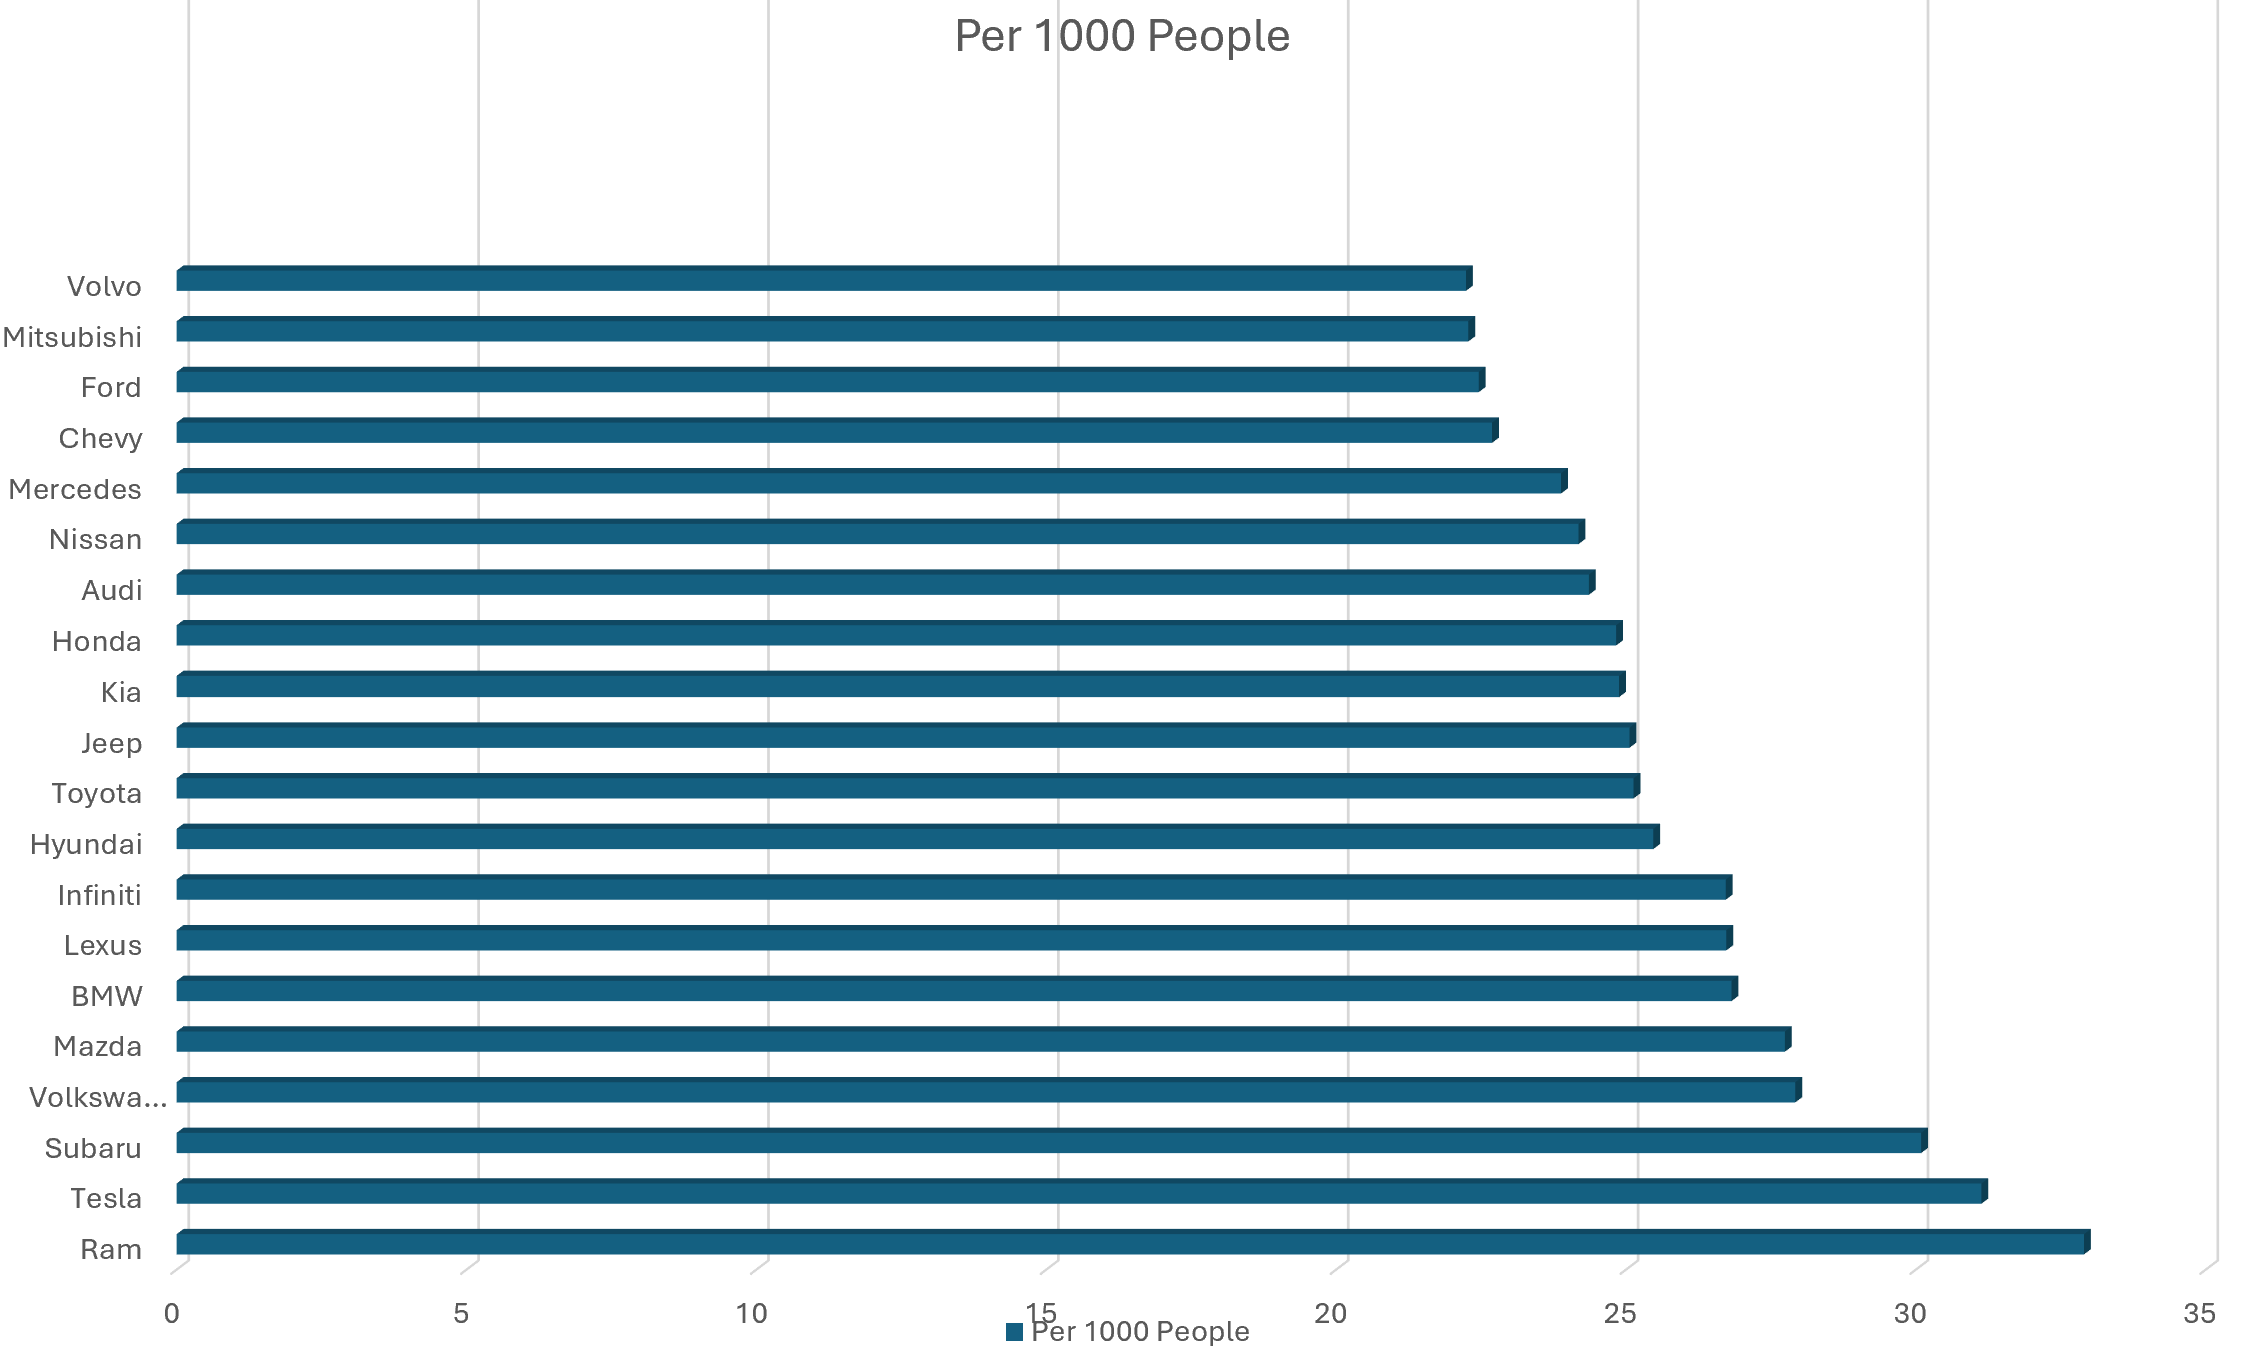
\includegraphics{Screenshot 2024-04-14 124410.png}

I created this graph in powerpoint using information from
https://www.lendingtree.com/ that shows the the most common car make in
accidents in the United States, It shows us that among the top 5 is Ram,
Tesla, Subaru, Volkswagen, and Mazda as the most common car makes to be
in an accident. But with this image alone doesn't tell us much. It only
tells us the most common makes and not other information such as where
the accidents happen?, who was the driver?, was the driver under the
influence of any substances? and many other important information that
is not shown here. But this is a 1st step and one of many in order to
reach my end goal of the most common characteristics of a car accident.

\hypertarget{background-and-related-work}{%
\subsection{Background and Related
Work}\label{background-and-related-work}}

Source:
https://www.nytimes.com/2023/12/11/briefing/us-traffic-deaths.html\\
\strut \\
In this article it reviews the fact that since the automotive the number
of accidents has steady decrease over the past century. But in recently
years only the untied states saw a increase in deaths with the
involvement of a motor vehicle while others like south Korea and Canada
is still seeing a decline or flattening out. This article addresses some
factors that could contribute to this such as cell phone culture, lack
of walk able spaces, and substances that hinders the drivers judgement.
This article attempts to create an insight that is similar to mine on
what is causing these crashes to happen and what could be done about it.

\hypertarget{data-processing}{%
\subsection{Data Processing}\label{data-processing}}

This data set was taking from https://www.kaggle.com/

This data set used records car accidents from 2003 to 2015 as well as
showing us the location of the crash, how many cars were involved, was
there any injuries, and what caused the crash to happened in the first
place

\textbf{Setting up data set for R}

\begin{Shaded}
\begin{Highlighting}[]
\FunctionTok{library}\NormalTok{(readr)}\CommentTok{\#packages needed}

\CommentTok{\# Read the CSV file into a data frame}
\NormalTok{df }\OtherTok{\textless{}{-}} \FunctionTok{read.csv}\NormalTok{(}\StringTok{"https://raw.githubusercontent.com/andydagao/380project/main/Copy\%20of\%20new\%20dataset.csv"}\NormalTok{, }\AttributeTok{sep=}\StringTok{","}\NormalTok{)}
\end{Highlighting}
\end{Shaded}

\textbf{Cleaning data set}

\begin{Shaded}
\begin{Highlighting}[]
\CommentTok{\#removing rows where it has NA}
\NormalTok{df }\OtherTok{\textless{}{-}} \FunctionTok{na.omit}\NormalTok{(df)}

\CommentTok{\#setting column names to lowercase}
\FunctionTok{names}\NormalTok{(df) }\OtherTok{\textless{}{-}} \FunctionTok{tolower}\NormalTok{(}\FunctionTok{names}\NormalTok{(df))}

\CommentTok{\#replaceing every . with \_}
\FunctionTok{names}\NormalTok{(df) }\OtherTok{\textless{}{-}} \FunctionTok{gsub}\NormalTok{(}\StringTok{"}\SpecialCharTok{\textbackslash{}\textbackslash{}}\StringTok{."}\NormalTok{, }\StringTok{"\_"}\NormalTok{, }\FunctionTok{names}\NormalTok{(df))}

\CommentTok{\#renaming weekend column}
\FunctionTok{names}\NormalTok{(df)[}\FunctionTok{names}\NormalTok{(df) }\SpecialCharTok{==} \StringTok{"weekend\_"}\NormalTok{] }\OtherTok{\textless{}{-}} \StringTok{"weekend"}
\end{Highlighting}
\end{Shaded}

\textbf{Statistics}

\begin{Shaded}
\begin{Highlighting}[]
\FunctionTok{library}\NormalTok{(ggplot2)}\CommentTok{\# library needed}

\CommentTok{\#bar grapg of the collusion type and the injuries reported from them}
\FunctionTok{ggplot}\NormalTok{(df, }\FunctionTok{aes}\NormalTok{(}\AttributeTok{x =}\NormalTok{ collision\_type, }\AttributeTok{fill =}\NormalTok{ injury\_type)) }\SpecialCharTok{+}
  \FunctionTok{geom\_bar}\NormalTok{()}
\end{Highlighting}
\end{Shaded}

\begin{figure}[H]

{\centering 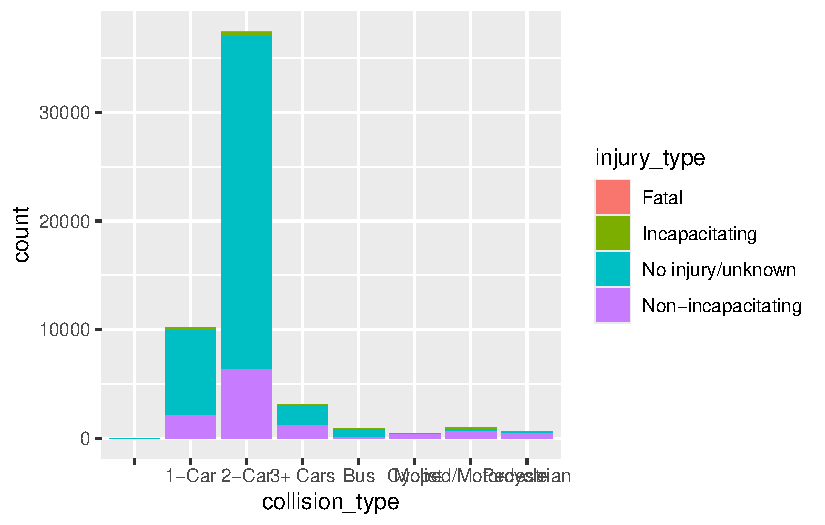
\includegraphics{380projectEDA_files/figure-pdf/unnamed-chunk-4-1.pdf}

}

\end{figure}

As we can see from this bar graph accidents involving 2 cars is
significantly higher than any of the rest with the runner up of only
being 1 car accidents is not even a 3rd of accidents involving 2 cars.
But thankfully we can see that most of the accidents resulted in no
injuries or life threatening

\begin{Shaded}
\begin{Highlighting}[]
\CommentTok{\#package needed}
\FunctionTok{library}\NormalTok{(dplyr)}
\end{Highlighting}
\end{Shaded}

\begin{verbatim}

Attaching package: 'dplyr'
\end{verbatim}

\begin{verbatim}
The following objects are masked from 'package:stats':

    filter, lag
\end{verbatim}

\begin{verbatim}
The following objects are masked from 'package:base':

    intersect, setdiff, setequal, union
\end{verbatim}

\begin{Shaded}
\begin{Highlighting}[]
\CommentTok{\#top causes for crashes}
\NormalTok{top5reasons }\OtherTok{\textless{}{-}}\NormalTok{ df }\SpecialCharTok{\%\textgreater{}\%}
  \FunctionTok{select}\NormalTok{(primary\_factor) }\SpecialCharTok{\%\textgreater{}\%}\CommentTok{\#select the variable of intrest}
  \FunctionTok{count}\NormalTok{(primary\_factor) }\SpecialCharTok{\%\textgreater{}\%}\CommentTok{\#count frequency }
  \FunctionTok{arrange}\NormalTok{(}\FunctionTok{desc}\NormalTok{(n))}\SpecialCharTok{\%\textgreater{}\%}\CommentTok{\#arrange from highest to lowest}
  \FunctionTok{head}\NormalTok{(}\DecValTok{5}\NormalTok{)}\CommentTok{\#get top 5 results}

\NormalTok{top5reasons}
\end{Highlighting}
\end{Shaded}

\begin{verbatim}
                         primary_factor     n
1         FAILURE TO YIELD RIGHT OF WAY 11176
2                 FOLLOWING TOO CLOSELY  7345
3 OTHER (DRIVER) - EXPLAIN IN NARRATIVE  6079
4                        UNSAFE BACKING  5168
5                    RAN OFF ROAD RIGHT  2919
\end{verbatim}

As we can see here the top 5 causes of accidents with the failure to
yield the right of way being the most common way that accidents occur.
Others include following to closely, Other(which could be anything),
unsafe backing, or ran off road.

Some issues could be easily fix such as unsafe backing which can be
solved with more sensors and cameras installed which can prevent such
situations from happening, others such as failure to yield may be more
difficult because it all depends on the driver's ability



\end{document}
